\documentclass[pdftex,12pt,a4paper]{report}
\usepackage{dbstmpl}
\usepackage{subfigure}

% Hier die eigenen Daten eintragen
\global\arbeit{Master's Thesis}
\global\titel{Detecting Global Correlated Clusters using Hough Transform through Locally Dense Correlations}
\global\bearbeiter{Long Mathias Yan}
\global\betreuer{Daniyal Kazempour}
\global\aufgabensteller{Dr. Peer Kr"oger}
\global\abgabetermin{14. November 2019}
\global\ort{Munich}
\global\fach{Computer Science}

\begin{document}

% Deckblatt
\deckblatt

% Erklaerung fuer das Pruefungsamt
\erklaerung

% Zusammenfassung
\begin{abstract}
Dieses Dokument dient als Muster f"ur die Ausarbeitung einer \the\arbeit\
an der Lehr- und Forschungseinheit f"ur Datenbanksysteme am Institut f"ur
Informatik der LMU M"unchen.
\end{abstract}

% Inhaltsverzeichnis
\tableofcontents

% Hier beginnt der eigentliche Text
\chapter{Introduction}\label{ch:intro}

In the midst of the fast-paced advancements in data processing and data acquisition, we currently are living in the age of increasing data abundance. While significant improvements in computing power enabled feasible information extraction processes, created the data-centric business practice and opened new possibilities in research in the first place, the concurrent rising acceptance of data collecting technologies and the hunger for more data in hopes for later use, rapidly increased and overtook the processible amount of data. 
% In the midst of the fast-paced advancements in data processing and even faster-paced data acquisition, we currently are living in the world and age of increasing data abundance. While significant improvements in computing power enabled feasible information extraction processes, created the data-centric business practice and opened new possibilities in research in the first place, the concurrent rising acceptance of data collecting technologies and the hunger for more data in hopes for later use, rapidly increased and overtook the processible amount of data. 
%  driven by e.g. increasingly powerful smart devices and other user behaviour tracking practices, increased the amount of data sources rapidly,
%Therefore even with an abundance of data the actual problem of information scarcity still applies.

This raw data often is present in the form of vast amounts of observations consisting of several features represented as numerical values and, thus, is hardly comprehensible for human insight or intuition. Without a 
procedure to extract meaningful information out of the data, this data abundance would be mostly useless for immediate human processing. One way to cope with this issue is the manual labelling of each observation. by human hand, which however obviously is getting more and more unrealistic since with the increasing amounts of data this task is getting inefficient and/or even infeasible. Therefore an automated method to extract relevant information is becoming essential to analyzing the exploding amounts of data. %To tackle this problem, there has been done much research in the fields of Deep- and Unsupervised Learning.

To deal with this problem, there has been lots of different approaches.
If the actual relevant features are not required and are just the means to achieve a goal, the analyzing task can be solved via implicit feature engineering, where it is assumed that the analyzing model learns relevant features by itself.
However if not, the analyzing task can be approached via unsupervised knowledge discovery processes, with goals such as a segmentation of data sets by some shared attributes, a simplification of data sets by aggregating variables with similarity or the detection of anomalies or correlations.

In tasks working with high-dimensional data sets, such as genome analysis in biology/medicine and text analysis in \gls{nlp}, it is particularly interesting, which \textit{features} play important roles in characterizing clusters. This task is called subspace clustering. In the special case of an additional interest in how the important features relate to each other, the task of \textit{correlation clustering} arises.

The problem with existing subspace and correlation clustering approaches is, that they are restricted to a given scope, either local or global, and do not have the capabilities to find the opposite scopes' result. This is inconvenient and limits the thorough evaluation of clusterings if both scopes are of interest. Our goal is to combine existing clustering paradigms to create a correlation clustering algorithm for both scopes simultaneously.

% does not restrict itself to the economic field but is apparent in various fields of science, such as


% This work in particular aims to tackle the
% In this work, we focus on an unsupervised solution for this problem. Namely, we propose a novel algorithm, which combines two different concepts to get a universal clustering of the data.

% \acrfull{cash} is cool, however its complexity is $\mathcal{O}(n^2)$.
% We try to do it better by using a density-based approach to prune away irrelevant points and noise.

\section{Problem Statement}
Our proposal is a correlation clustering algorithm, which builds upon an existing local classical clustering approach and a global correlation clustering approach. It combines those into a more exhaustive algorithm which can give a more comprehensive insight, notably a simultaneously local and global view, onto the applied data while additionally providing a similar performance compared to the global correlation clustering approach. In particular, we first apply a density-based approach onto the data sets to filter out relevant subintervals of the original data space (not to be confused with subspaces) and evaluate those by applying a correlation clustering algorithm based on the Hough transform. Those local results are then stitched together and used to reevaluate previously (falsely) pruned points, to get a complete evaluation of every point of the data set. With this approach, we receive a labelling of a local view and also a global view of the points. 

\section{Structure of the Thesis}
The structure of this thesis is organized as follows:

First off, \textit{\autoref{ch:intro}} introduces/illustrates the motivation of our thesis using tasks/problems from various fields of the current age.
\textit{\hyperref[ch:overview]{Chapter~\ref*{ch:overview}}} gives a general overview of the terminology of clustering, provides a general structure of its different archetypes and leads the reader towards our unique use case.
\textit{\hyperref[sec:Related Work]{Chapter~\ref*{sec:Related Work}}} covers a collection of related works not able to cluster in the desired manner with regards to correlation clustering and introduces components necessary to our algorithm to tackle these problems.
In \textit{\autoref{ch:Methods}}, we provide an in-depth explanation of our algorithm's core components and give an extensive view of the separate steps of our novel approach.
\textit{\hyperref[ch:evaluation]{Chapter~\ref*{ch:evaluation}}} examines our algorithm's runtime, and clustering performance with regards to different data set characteristics, such as numbers of data objects, amount of noise and dimensionality, and compares its result to its ancestor/peer \acrshort{cash}.
To wrap up this work, \textit{\autoref{ch:conclusion}} concludes this thesis by summarizing the current state of research in the field of correlation clustering, and based on the results, aims to categorize our approach within this field. As an outlook \textit{\autoref{ch:futurework}} points out possible future work.

% First off \textit{\autoref{ch:intro}} introduces/illustrates the motivation of our thesis using tasks/problems from various fields, e.g. biology, medicine, economy, etc., of the current age.
% \textit{\hyperref[ch:overview]{Chapter~\ref*{ch:overview}}} gives a general overview of the terminology of clustering, provides a general structure of the different archetypes and leads the reader towards our special type of clustering where our use case is relevant.
% \textit{\hyperref[sec:Related Work]{Chapter~\ref*{sec:Related Work}}} covers a collection of related works not able to cluster in the desired manner with regards to correlation clustering and introduces components necessary to our algorithm to tackle these problems.
% In \textit{\autoref{ch:Methods}} we provide an in depth explanation of our algorithms core components and give an extensive view to the separate steps of our novel approach.
% \textit{\hyperref[ch:evaluation]{Chapter~\ref*{ch:evaluation}}} examines our algorithms runtime and clustering performance with regards to different data set characteristics, such as numbers of data objects, amount of noise and dimensionality, and compares its result to its ancestor/peer \acrshort{cash}.
% To wrap up this work \textit{\autoref{ch:conclusion}} concludes this thesis by summarizing the current state of research in the field of correlation clustering, and based on the results, aims to categorize our approach within this field. As an outlook \textit{\autoref{ch:futurework}} points out possible future work.

% Note that in this thesis \textit{subspaces} and \textit{subspace clusters}, except in \autoref{sec:clu} or unless explicitly stated, always refer to \textit{linear} arbitrarily oriented subspaces/correlations and its clusters. We also use \textit{subspace clustering} and \textit{correlation clustering} interchangeably.
% \todor{Notiz behalten?}
\chapter{Related Work}
\label{sec:Related Work}
% This chapter introduces some foundational work on density-based and subspace/correlation clustering and aims to give an intuitive insight into existing approaches to solve the problem of subspace clustering. We also elaborate, where these existing approaches lack in ability and capability and show some of the current optimization approaches.
This chapter introduces some foundational work on subspace/correlation clustering and aims to give an intuitive insight into existing approaches to solve the problem of subspace clustering. In particular the elaboration on the related work is twofold: we introduce subspace/correlation extraction/clustering methods such as basic \acrshort{pca} and \acrshort{orclus}, and additionally expand on algorithms which augment the subspace clustering method such as \acrshort{dbscan} in \acrshort{4c}. We also elaborate, where these existing approaches lack in ability and capability and show some of the current optimization approaches.

Since sections \nameref{sec:houghintro}, \nameref{sec:cashintro}, \nameref{sec:dbscanintro} and \nameref{sec:OPTICSintro} are essential components to our work they will be elaborated in greater detail in the chapter \nameref{sec:Foundations}

\section{Existing Subspace Clustering Algorithms}
There are many approaches for detecting relevant subspaces in data, generally grouped to either finding axis-parallel or arbitrarily oriented subspaces. Our work in particular focuses on the extraction of the second type of subspaces, which obviously proves to be a more challenging task since it encompasses the problem of axis-parallel subspace clustering\todor{the first type}. This task is also referred to as \textit{Correlation Clustering}. 

This section introduces some existing correlation clustering algorithms and illustrates \todor{choose one: demonstrates/analyzes/explains/illustrates/points out} their advantages and disadvantages and elaborates on their suitability for our idea.

\subsection{PCA}
A common way to filter out relevant features/subspaces in high dimensional data is the application of feature selection/dimensionality reduction. One of the oldest and most widely used methods is the \gls{pca}. It is a statistical approach which uses an orthogonal transformation to transform the original basis of a $d$-dimensional data space $DS$ to a basis built upon $d$ so called \textit{Principal Components} $PC$, where the first Principal Components $PC_1$ is a vector which describes the largest percentage of explained variance in $DS$. Each Principal Component $PC_j$ next in order $j,\dotsc,d$ is orthogonal to the previous ones $PC_i, i<j$ and is ordered by the next highest explained variance. Mathematically finding the Principal Components in a data set $DS$ boils down to solving its eigendecomposition \todor{nicht ganz korrekt. eigendecomp von cov(x)}, where the eigenvector with the highest corresponding eigenvalue represents the first Principal Component and the second highest the second Principal Component, etc\cite{pcawold1987principal}. For further details to the calculation \textcite{pcamljolliffe1986principal} offers a short and intuitive step-by-step explanation.
Unfortunately the extraction of relevant features via \gls{pca} is rarely of use for clustering problems. Unmodified \gls{pca} is global in nature and can only compute one subspace of the original data space and does not address the problem of \textit{local feature relevance} or \textit{local feature correlation}, which essentially states, that different clusters in data space can exist in different subspaces\cite{kriegel2009clustering} (c.f. \cite{PCAshlens2014tutorial}). \todor{PCA besser erklaeren}

\todob{PCA own fig}
\begin{figure}
    \centering
    \begin{minipage}[t]{.5\textwidth}
      \centering  
      \captionsetup{width=.9\linewidth}
      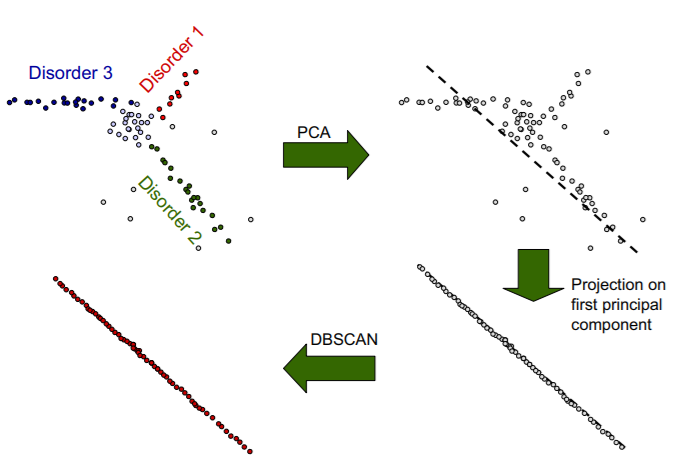
\includegraphics[width=.9\textwidth]{figures/pcalocalfeat1.png}
      \captionof*{figure}{a) First}
      \label{fig:test1}
    \end{minipage}%
    \begin{minipage}[t]{.5\textwidth}
      \centering
      \captionsetup{width=.9\linewidth}
      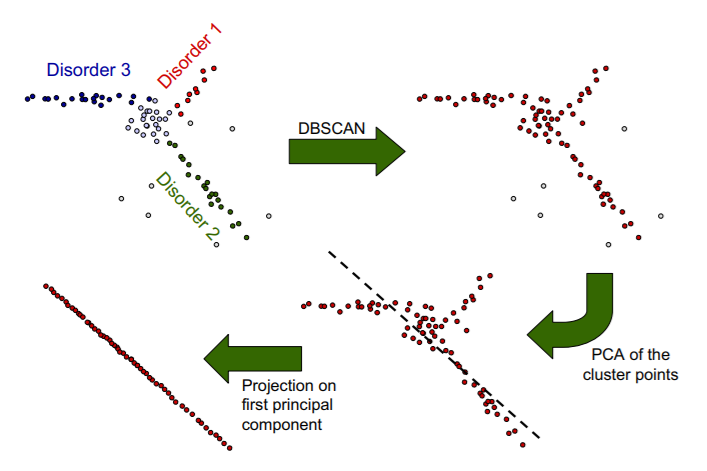
\includegraphics[width=.9\textwidth]{figures/pcalocalfeat2.png}
      \captionof*{figure}{b) Second}
      \label{fig:test2}
    \end{minipage}
    \caption{lazy}
    \label{fig:localfeatrelevance}
\end{figure}

\subsection{ORCLUS}
Since \gls{pca} only provides a global view of the correlations in data space and does not address the local feature relevance, \gls{orclus} attempts to enforce \gls{pca} to only consider local segments of the data space via a $k$-Means-like approach. 

To find $k$ many $l$-dimensional subspace clusters in a $d$-dimensional data space, \gls{orclus} first initializes $k_c, k_c > k$ seeds $s_i$ as centroids and applies the default (euclidean) $k$-Means to partition the data space into $k_c$ clusters $C_i$ with $i \in \{1,\dotsc,k_c\}$. After that iteratively all points are reassigned to the new cluster centroids via a modified distance function based on a subset of $l_c, l\leq l_c \leq d$ weak eigenvectors/principal components $\varepsilon_i$ of each cluster $c_i$. This subset of $l_c$ eigenvectors represents the current dimensionality of the cluster in each iteration and is adapted such that at the end of all iterations $l_c=l$ holds. Additionally at the end of each iteration the closest pair (in terms of average modified distance) of clusters are merged together resulting in $k_c = k_c-1$ clusters afterwards. This reassigning-merging process is repeated until $k_c = k$ holds. Due to the localized view on the single partitions \gls{orclus} is considered as a local correlation clustering algorithm\cite{orclusaggarwal2000finding}.

As an adopter of $k$-Means and \gls{pca}, \gls{orclus} however also comes with its components disadvantages. It relies on $k$, which is difficult to determine, does not handle noise and outliers, and extracts the subspaces based on the clusters eigenvectors, which are not necessarily a good representation of the members distribution (c.f. \autoref{fig:localfeatrelevance}).


\subsection{4C}\label{ssec:4c}
Analogous to \gls{orclus}, \gls{4c} also aims to construct a localized view of the data space. This time however a density-based approach is used. 

To find $\lambda$-dimensional subspace clusters in a $d$-dimensional space, \gls{4c} employs a customized/an extended \acrshort{dbscan} by modifying parts of the density criterion. 
% After clustering the data space into usual dense clusters, each cluster is reevaluated according to its variance. This is done by applying \gls{pca} to the locally dense cluster. If the $d-\lambda$ smallest eigenvectors of the cluster are not close enough to threshold $\delta \approx 0$
Instead of uniformly assessing the neighborhood in all directions, the modified density criterion biases the neighborhood query according to the neighborhoods variance. First, only dense candidates/core points, that have a maximum of $\lambda$ eigenvalues $\varepsilon_i > \delta$ in its neighborhood, are considered. $\delta$ denotes a threshold for a variance in unrelated dimensions. Secondly, these points are grouped together based on their membership in each others modified neighborhood. These resulting clusters are, much like \gls{orclus}, also based on a localized view (this time dense clusters) and therefore also only able to create a local correlation clustering\cite{4cbohm2004computing}. A detailed explanation to the original \acrshort{dbscan} is found in \autoref{ssec:DBSCANindepth}.

In contrast to \gls{orclus}, \gls{4c} enables the handling of noise and outliers. The modification of the density criterion essentially promotes a density-based propagation of the cluster biased towards the found local correlations, but due to the lose constraint of a maximum amount of eigenvalues, \gls{4c} just finds close to $lambda$-dimensional clusters.

\subsection{COPAC}
\gls{copac}, like \gls{4c}, also uses an approach based on \acrshort{dbscan}, however this time the modified \acrshort{dbscan} artificially only considers distances related to the correlating (global) hyperplane and thus creates a global correlation clustering. 

Instead of determining each points dimensionality according to its dense neighborhood (c.f. \autoref{ssec:4c}), \gls{copac} first assigns each point its \textit{local correlation dimensionality} $\lambda$, which denotes the smallest amount of eigenvectors explaining at least $\alpha$ percent of the $k$-nearest neighbors variance, and partitions them based on $\lambda$. Secondly, clusters each partition is processed with a modified \acrshort{dbscan}. This modified \acrshort{dbscan} now only considers the $d-\lambda$ weakest eigenvectors of the k-nearest neighbors in the distance functions and therefore clusters each partition based on the distance to the strong eigenvectors/correlations.

Due to the inital partitioning based on the local correlation dimensionality $\lambda$, \gls{copac} does not need a parameter to detect a specific dimensional correlation, but instead simultaneously finds correlation clusters of arbitrary dimensions. The difficulties here rely on the choice of the parameter $k$, which at least can be constraint to $k>d$
\todor{moechte eigtl nicht sagen, dass das gut oder schlecht ist, vllt will man ja gezielt nach einer dimensionalitaet suchen?}\\


% \subsection{HiCO and ERiC} \todor{passt so halb rein, bau ja n fulldim hierarchy}
% (Global) Correlation Clustering, other algorithms so far (ORCLUS \cite{orclusaggarwal2000finding}, LMCLUS \cite{}, 4C, HiCO, ERiC)[1]

% Since many of the existing correlation clustering algorithms rely on \gls{pca} they also come with its limitations. 

\section{Hough Transformation}\label{sec:houghintro}
The Hough Transform originally was introduced by \textcite{houghOriginal1962method} and extended by \textcite{rosenfeld1969picture} in the field of computer vision for edge detection\cite{houghhistoryhart2009hough}. The initial purpose of the Hough transform was a technique to detect colinear points in an image space but has since then found various other applications in fields like image processing/analysis~\cite{rosenfeld1969picture,ballard1981generalizing}, computer vision~\cite{davies2004machine} and subspace clustering\cite{CASHachtert2008robust}.

The basic idea of the Hough transform is the transformation of all points $p_i = (x_i,y_i)$ in a 2-dimensional image space $\mathcal{D} \subseteq \R^2$ to functions $f_{p_i}$ in a 2-dimensional parameter space $\mathcal{P} \subseteq \R^2$, also known as Hough space\cite{illingworth1988survey}. This is can be done by e.g. taking a representation of a point $p$ as all of its concurrent lines $y_p = m \cdot x_p + t$ and rearranging it to $m_{p} = - \frac{1}{x_p} \cdot t_{p} + \frac{y_p}{x_p}$ which produces a straight with slope $m$ and y-intersect $t$ in a $(m,t)$-parameter space. Since each point in parameter space represents a particular $(m,t)$-setting, multiple functions close to each other implies that their respective points have similar $(m,t)$-settings as well. The correlation clustering objective therefore transforms to a density-based clustering objective in parameter space, with the added benefit of being able to detect correlating points regardless of their distance to each other in data space. This property is exploited by e.g. evaluating the whole parameter space in a grid with a voting scheme or by smartly splitting the parameter space in \autoref{sec:houghintro} to detect linear correlations. 
\todor{Ich plagiere mich selbst. 1zu1 aus unterem abschnitt}
% \begin{figure}
%     \centering
%     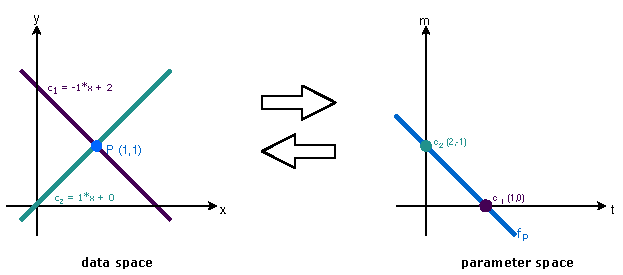
\includegraphics{figures/HoughMXT.pdf}
%     \caption{Caption}
%     \label{fig:houghmxt}
% \end{figure}\todor{eher keine bilder in related work}

\section{CASH}\label{sec:cashintro}
The global correlation clustering algorithm \gls{cash} extends the use case of the Hough Transformation to the detection of arbitrary-dimensional subspaces by augmenting the initial rigid 2-dimensional definition to a multi-dimensional one. 

Furthermore \gls{cash} introduces a improved search strategy for detecting regions of high intersections in parameter space to improve the efficiency compared to the basic grid search \cite{CASHachtert2008global}. Instead of doing an extensive count operation/accumulation of intersections over a fixed interval, \gls{cash} successively splits the whole parameter space by its axes and only further evaluates the split hypercuboids if they contain enough intersections. This is repeated until a certain count of splits is reached and only then hypercuboids with enough intersections are considered as linear correlations. 

Since our work focuses on ``\textit{Detecting Global Correlated Clusters using Hough Transform through Locally Dense Correlations}'', we use \gls{cash} to cope with multi-dimensional data and detect our locally dense correlations. Additionally we will use \gls{cash} as a performance baseline for our descendant algorithm to compare them in a global setting.
A more profound explanation to the transformation and its usage in \gls{cash} will be given in \autoref{ssec:houghindepth}.

% Please add the following required packages to your document preamble:
% \usepackage{booktabs}
% \usepackage{graphicx}
\begin{table}[]
\centering
\resizebox{\textwidth}{!}{%
\begin{tabular}{@{}|l|c|c|c|l|@{}}
\toprule
\textbf{Algorithm}                 & \textbf{\begin{tabular}[c]{@{}c@{}}Local \\ Subspaces\end{tabular}} & \textbf{\begin{tabular}[c]{@{}c@{}}Global \\ Subspaces\end{tabular}} & \textbf{\begin{tabular}[c]{@{}c@{}}Global \\ Subspaces\end{tabular}} & \textbf{Notes}                                                                                                                                                                                                   \\ \midrule
\acrshort{pca}    & \xmark    & \cmark     & \xmark      & \tabitem Only handles single or orthogonal correlations well                                                                                                                                                              \\ \midrule
\acrshort{orclus} & \cmark    & \xmark     & \xmark      & \tabitem Combines \acrshort{pca} with a $k$-Means-like approach                                                                                                                                          \\ \midrule
\acrshort{4c}     & \cmark    & \xmark     & \xmark      & \tabitem Combines \acrshort{pca} with a density-based approach                                                                                                                                           \\ \midrule
\acrshort{copac}  & \xmark    & \cmark     & \xmark      & \begin{tabular}[c]{@{}l@{}}\tabitem Similar to \acrshort{4c}\\ \tabitem Combines \acrshort{pca} with a density-based approach\end{tabular}                                                       \\ \midrule
\acrshort{hico}   & \xmark    & \cmark     & \cmark      & \begin{tabular}[c]{@{}l@{}}\tabitem Creates a Correlation distance ordering similar to \acrshort{optics},\\ \tabitem creates a tree-like hierarchy\end{tabular}                                                   \\ \midrule
\acrshort{eric}   & \xmark    & \cmark     & \cmark      & \begin{tabular}[c]{@{}l@{}}\tabitem Similar to \acrshort{hico}\\ \tabitem Creates a Correlation distance ordering similar to \acrshort{optics}, \\ \quad \ but creates a graph-like hierarchy\end{tabular} \\ \midrule
\acrshort{cash}   & \xmark    & \cmark     & \cmark      & \tabitem Uses the Hough-Transform to                                                                                                                                                                                      \\ \bottomrule
\end{tabular}%
}
\caption{}
\label{tab:corrcluchar}
\end{table}

\section{DBSCAN}\label{sec:dbscanintro}
\citeauthor{DBSCANEKSX96} created a foundational algorithm with \gls{dbscan}. With over 16000 citations on google scholar as of December 2019 it is one of the most influential works created in the field of density-based clustering and a basis to many clustering approaches, not only restricted to density-based clustering. 

As its name reveals it is an algorithm which detects points in dense vicinity and groups them together. For a measure of density \gls{dbscan} utilizes two parameters. One to specify the minimum amount of neighboring points in a close vicinity and one to specify the range/radius of that vicinity. Points fulfilling these conditions are called \textit{core points} and represent the dense \textit{core} of a cluster. The border of a dense cluster is composed of \textit{border points}. They are points which themselves do not possess a dense neighborhood but are still in the vicinity of core points. 

In contrast to $k$-means-like partitioning clustering\cite{kmeansmacqueen1967some}, \gls{dbscan} is able to find not only non-convex shapes, but also any arbitrary shape of a particular density. Since these arbitrary shaped clusters preserves their correlations and our goal is the assembly of locally dense correlations to global correlations, we expect to obtain good results by partitioning our data space via a density-based algorithm.

\section{OPTICS}\label{sec:OPTICSintro}
A disadvantage of \gls{dbscan} is its dependence on a fixed global parameter setting defining the \textit{minimal} detectable density. Assuming a global linear correlation to have low fluctuations in variance and different global linear correlations having various other variances\todor{can i assume this? i have to do some assumptions right?}, finding clusters with single densities would be more advantageous to our algorithm. We therefore adopted the use of \gls{optics} instead, an improvement/extension of \gls{dbscan}, which enables us to extract single densities more accurately \cite{opticsankerst1999optics}. Since \gls{dbscan} and \gls{optics} are the foundations of the partitioning step we will give a more comprehensive explanations to those two algorithms as well (c.f. \autoref{ssec:DBSCANindepth} and \autoref{ssec:OPTICSindepth}).
% Maybe OPTICS? DIRECTLY COPIED OUT OF \cite{ankerst1999optics}
%  First, almost all clustering algorithms require values for input parameters which are hard to
% determine, especially for real-world data sets containing highdimensional objects. Second, the algorithms are very sensible to
% these parameter values, often producing very different partitionings of the data set even for slightly different parameter settings.
% Third, high-dimensional real-data sets often have a very skewed
% distribution that cannot be revealed by a clustering algorithm using only one global parameter setting. 

% \section{Current Optimization Approaches}
% (D-MASC\cite{kazempour2018d, kazempour2019galaxy}, A Galaxy of Correlations etc.) [0.5] \todor{DMASC ist eigtl nur related work zu CASH aber relevant fuer uns?}
    

\chapter{Methods}
\section{Mathematical and Algorithmic Foundations [4]}
\subsection{Hough Transformation [2]}
\subsection{CASH [1]}
\subsection{DBSCAN [1]}

\section{The Algorithm [5]}

\subsection{Finding Dense Clusters}
Find dense clusters using DBSCAN → elaborate on bounding boxes around dense areas [1]

\subsection{Finding Linear Correlations}
Apply CASH onto dense Clusters [2]

\subsection{Stitching}

Assembly of local linear correlations [2]
\chapter{Evaluation}
To measure the performance of our algorithm, we evaluated \todor{werden tests evaluiert, oder algorithmen?} it on custom synthetic \textit{labeled} data sets, generated via the method mentioned in \autoref{sec:datagen}, which serves as the \textit{groundtruth} of our data. Explicitly we compared our novel algorithm with its ancestor \gls{cash} in clustering and runtime performance in various settings we will mention later. Since clustering is an unsupervised setting and the different clustering algorithms do not label the clusters uniformly with the same schema/value, we chose to compare the clustering labels via the \gls{ari}\cite{hubert1985comparingari} and \gls{nmi}\cite{strehl2002clusternmi} score, which are invariant to the permutations of the labeling. Later in this chapter we review the available hyperparameters of our algorithm and, based on previously evaluated data, explain their impacts on the performance.

The algorithms and evaluation are implemented in \textit{python v3.7.4}. Each of the data sets locally dense correlations are uniquely labeled and previously pruned noise points relabeled to a nearby linear correlation if the point was within a certain vicinity from the correlation away. For the density-based clustering we applied \gls{optics} from \textit{scikit-learn v0.21.2}\cite{pedregosa2011scikit} and for the extraction of the correlations we utilized \gls{cash} from the data mining tool \textit{\gls{elki} v0.7.5}\cite{achtert2008elki}. 

% We defined the threshold of the vicinity as $jitter_{thres}$ which merges the noise points if the euclidean distance to a nearby linear correlation $distance_{point\rightarrow hyperplane} = \frac{\Vec{n}\cdot\Vec{x}+\delta}{|\Vec{n}|}$ is smaller than the threshold. These data sets are served as our \textit{groundtruth}. Based on these groundtruths we compared our local-global combining clustering approach's results with its ancestor \gls{cash}'s results in the accuracy of their labeling based on the \gls{ari} and \gls{nmi} score and its runtime performance.

\todor{reichen 2d veranschaulichungen? 3d is hard}

\section{Setup}\label{sec:setup}

Our test setups were conducted on $d$-dimensional synthetic data sets with four characteristic jittery $d-1$-dimensional correlations, i.e. partial, intersecting and/or parallel correlations. The tests consisted of the evaluation of the algorithms different behaviours w.r.t runtime, \gls{ari} and \gls{nmi} scoring for six different amounts of points/objects (1000, 2000, 4000, 8000, 16000, 32000), five different dimensionalities (2, 3, 4, 8, 16) and seven different levels of noise (0, 1, 5, 10, 25, 40, 80).

All following tests were executed in docker containers running on a Virtual Machine with an x86\_64 bit architecture, 48 CPUs (2 GHz) and 246GB RAM. 

\begin{figure}
    \centering
    \begin{minipage}[t]{.5\textwidth}
    \centering
    \captionsetup{width=.9\linewidth}
    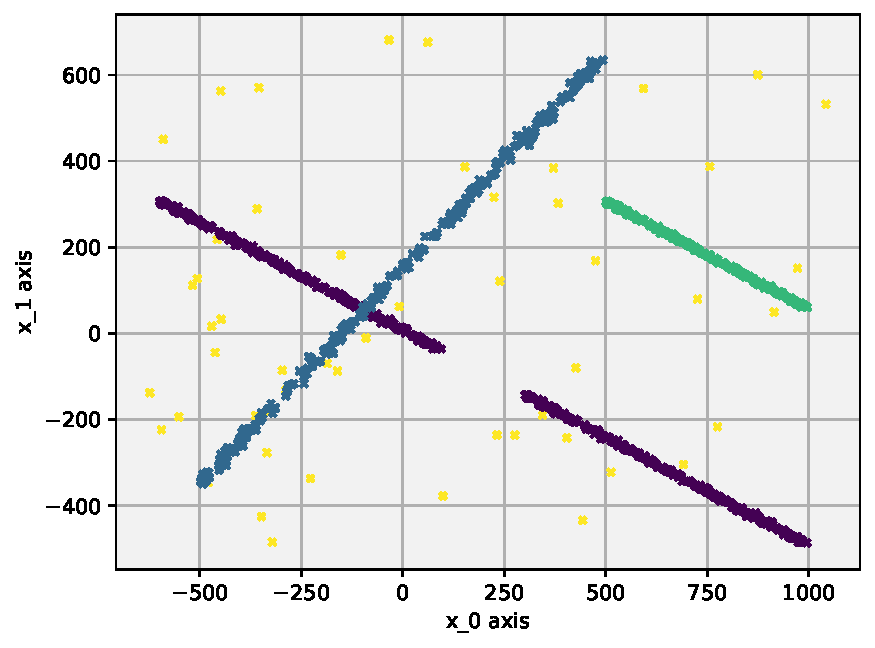
\includegraphics[width=\textwidth]{evalfigures/2DSetGrid.pdf}
    \captionof{figure}{Insight into clustering structure in 2D and 3D}
    \label{fig:my_label}
    \end{minipage}%
    \begin{minipage}[t]{.5\textwidth}
    \centering
    \captionsetup{width=.9\linewidth}
    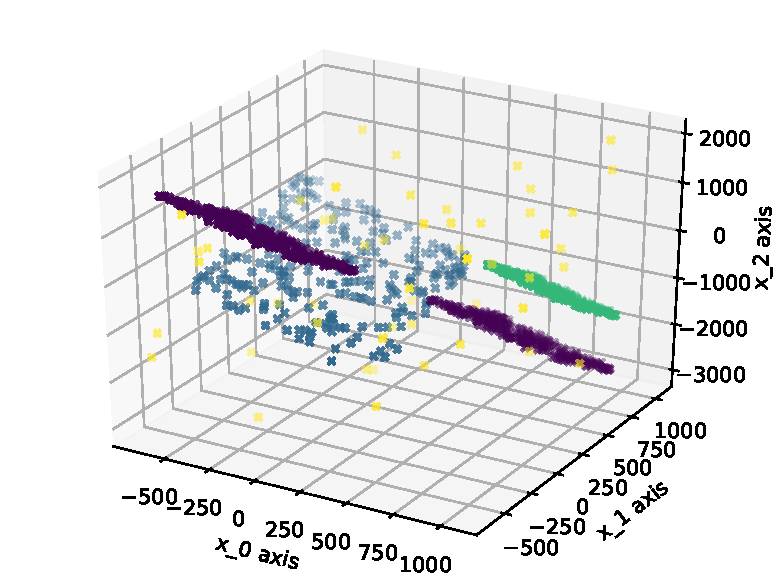
\includegraphics[width=\textwidth]{evalfigures/3DSet.pdf}
    \captionof{figure}{Insight into clustering structure in 2D and 3D}
    \label{fig:my_label}
    \end{minipage}%
\end{figure}

% The algorithms and evaluation are implemented in \textit{python v3.7.4}. Each of the data sets locally dense correlations are uniquely labeled and previously pruned noise points relabeled to a nearby linear correlation if the point was within a certain vicinity from the correlation away. For the density-based clustering we applied \gls{optics} from \textit{scikit-learn v0.21.2}\cite{pedregosa2011scikit} and for the extraction of the correlations we utilized \gls{cash} from the data mining tool \textit{\gls{elki} v0.7.5}\cite{achtert2008elki}. 

% (which data sets have been used? How many data objects? How many clusters? Which programming language and libraries? On which hardware?) [0.5]
\section{Performance}
 To evaluate the performance of our algorithm compared to \gls{cash} we performed up to 500 iterations of random parameter search on each data set while tracking runtime for a measure of efficiency and scoring the effectivity based on the \gls{ari} and \gls{nmi} score compared to our prelabeled groundtruth. However due to time constraints we bounded the maximal time for all iterations to a maximum of 24 hours. \todor{unsicher ob das rein soll}We’d like to note at this point that the current implementation may not satisfy the need to deliver a high performance with regards to the runtime, since we rely on \gls{elki}, which temporarily stores our necessary intermediate results to disk and therefore bottlenecks on I/O. For future work, we recommend to further research and elaborate on strategies to accelerate the execution time of our approach. 
 
\begin{table}[hb]
\centering
\resizebox{\textwidth}{!}{%
\begin{tabular}{@{}llll@{}}
\toprule
Test setting           & Dimensions & Noise in \% & \# of objects \\ \midrule
Increasing objects    & 3D         & 5           & -             \\
Increasing dimensions & -          & 5           & 10000         \\
Increasing noise      & 3D         & -           & 10000         \\ \bottomrule
\end{tabular}%
}
\caption{}
\label{tab:reducedsetup}
\end{table}
 
\subsection{Efficiency}
In context of efficiency we investigate the runtime performance of both local (our algorithm) and global (default \gls{cash}) by three different indications, namely number of objects, number of dimensions and amount of noise.

For the first aspect, we increased the data sets with regards to the number of objects. Here, we asked deliberately: what is the impact regarding the runtime if we modify the data set size?
And further: do we observe any differences between the original \gls{cash} algorithm and our approach? In theory we expect that our method yields similar results as \gls{cash}.

%  The evaluation of runtime performance measures the average runtime of the three different settings for both local (our algorithm) and global (default \gls{cash}) approaches. 

\begin{figure}[h]
    \centering
    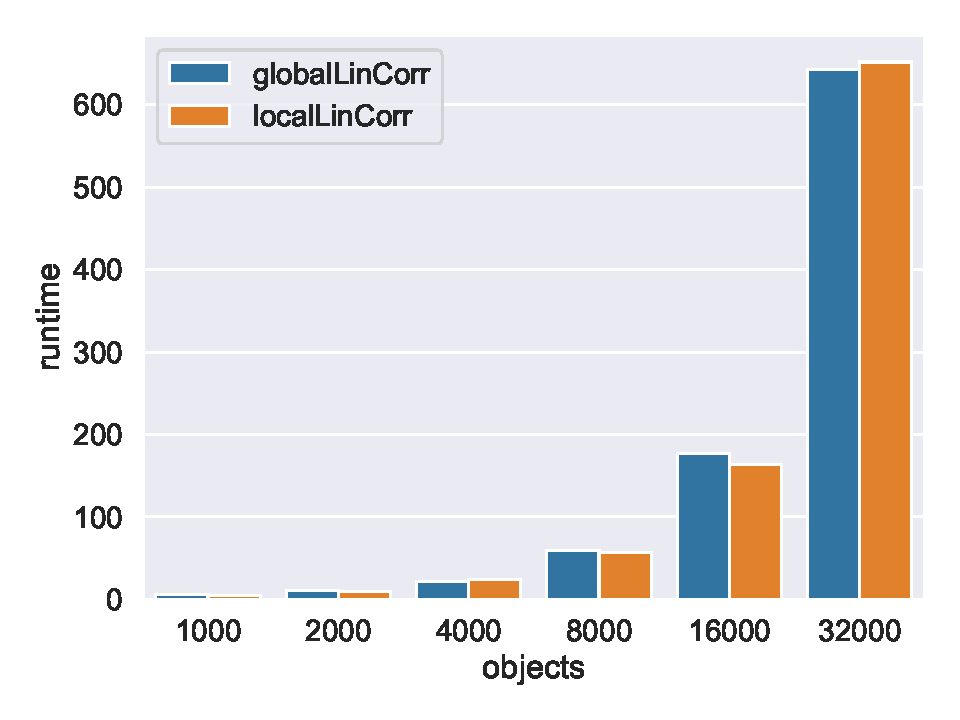
\includegraphics[width=0.8\textwidth]{evaluation/per_objects/Avg_Runtime_3D_N5_pobjects_bar.pdf}
    \caption{Caption}
    \label{fig:eval_per_objects}   
\end{figure}

\autoref{fig:eval_per_objects} shows the average runtime of both algorithms w.r.t. the \textit{number of objects} in 3-dimensional clusters of the data set. The data sets had a variable size of 1000, 2000, 4000, 8000, 16000 and 32000 number of objects with 5 percent noise respective to the data set size. Here our algorithm scales comparably to \gls{cash} and does not deteriorate in runtime performance even with higher numbers of objects even though the overhead of the partitioning, stitching and relabeling increases. This can be explained due to the shorter runtimes of the localized \gls{cash} processes, since the partitioning step reduces the amount of regions of interest in the parameter space of the Hough transform.\\

The second question regarding to efficiency is: How fast does our algorithm perform at different levels of noise? Is it comparable to the original \gls{cash}?. To assess the robustness of our algorithms efficiency against noise we compared the average runtimes of 500 iterations of both algorithms with respect to the amount of noise in the data space. Instead of modifying the total number of points of the whole data set, we now just evaluate the impact of different levels of noise percentage and compare the results of our approach with \gls{cash}s.

% of the average runtime w.r.t the different dimensionalities of the data space is depicted in \autoref{fig:eval_per_dim}.

\begin{figure}[h]
    \centering
        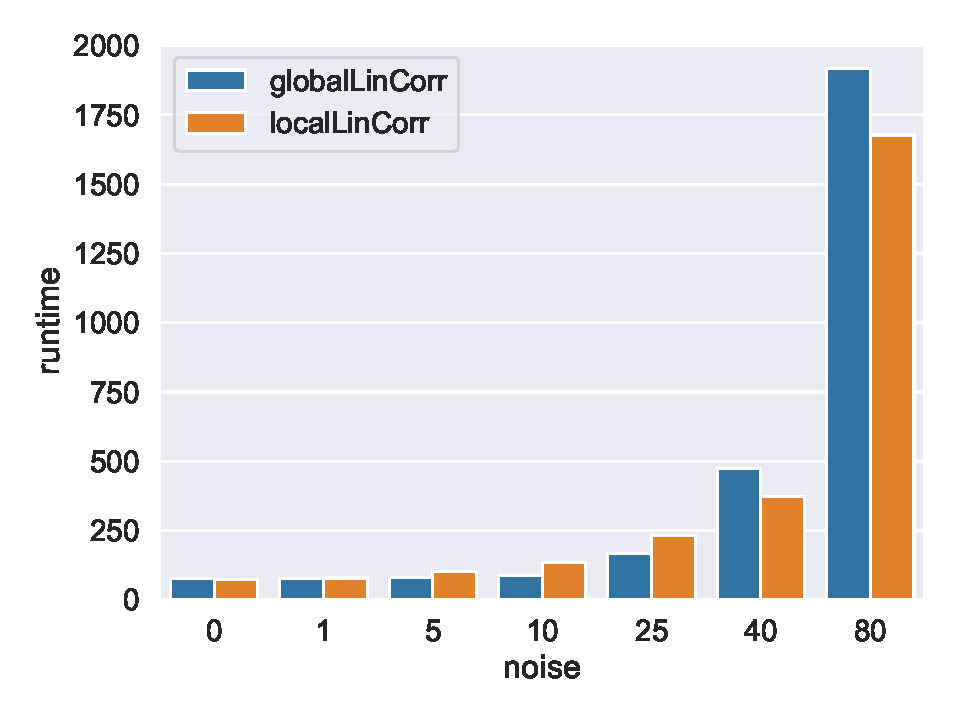
\includegraphics[width=0.8\textwidth]{evaluation/per_noise/Avg_Runtime_3D_O10000_pnoise_bar.pdf}
    \caption{Runtime in seconds w.r.t. the noise percentage}
    \label{fig:eval_per_noise}
\end{figure}

\autoref{fig:eval_per_noise} shows the average runtime of our algorithm with respect to the noise percentage of the data sets compared to the global approach. In this experiment our algorithms were evaluated on a 3-dimensional data set with 10000 points distributed among all clusters and seven different levels of noise percentage (0,1,5,10,25,40,80) on top of the initial data set. Note that noise points close enough to existing correlation clusters are relabeled to the respective cluster before evaluation which slightly skews the actual noise percentage in each data set.
As in the previous runtime measurements with regards to number of objects, the runtimes with respect to noise also remain stable on multiple levels compared to the global \gls{cash}. The overhead of the other components again is compensated by the quicker runtime of the partitioned \gls{cash}. At higher levels of noise (40 and 80 percent) it is even noticeable, that our approach gets a slight speed up compared to the global approach, since at these levels of noise the global cash will need to process more candidates in parameter space. In comparison our approach prunes away density-based noise first due to the partitioning step and leaves each localized \gls{cash} with comparably less candidates.
% At very low levels of noise both algorithms runtime remain stable. However increasing the noise further creates a gap in runtime results in favor of the global approach. This might be due to the overhead of the components increasing faster compared to the reduction in runtime of \gls{cash}, and second 

Our last runtime evaluation was conducted with regards to the dimensionality of the data set. Unlike in previous experiments, the data sets now change in \textit{space} instead of number of data objects. To keep a consistent comparable setting between the dimensionalities, we enforce our data set to be composed of similar four characteristic correlations, building a data space with partially split, intersecting and parallel $d-1$-dimensional hyperplanes. 
Note that runtimes dependent on dimensionality scale in $\mathcal{O}(2^d)$. Therefore the runtime figure with respect to the dimensionality scales logarithmically on the y-axis. Due to time constraints we set an upper bound for the runtime and restricted each run to a maximum of two hours. \todor{soll das rein?}

\begin{figure}[h]
    \centering
        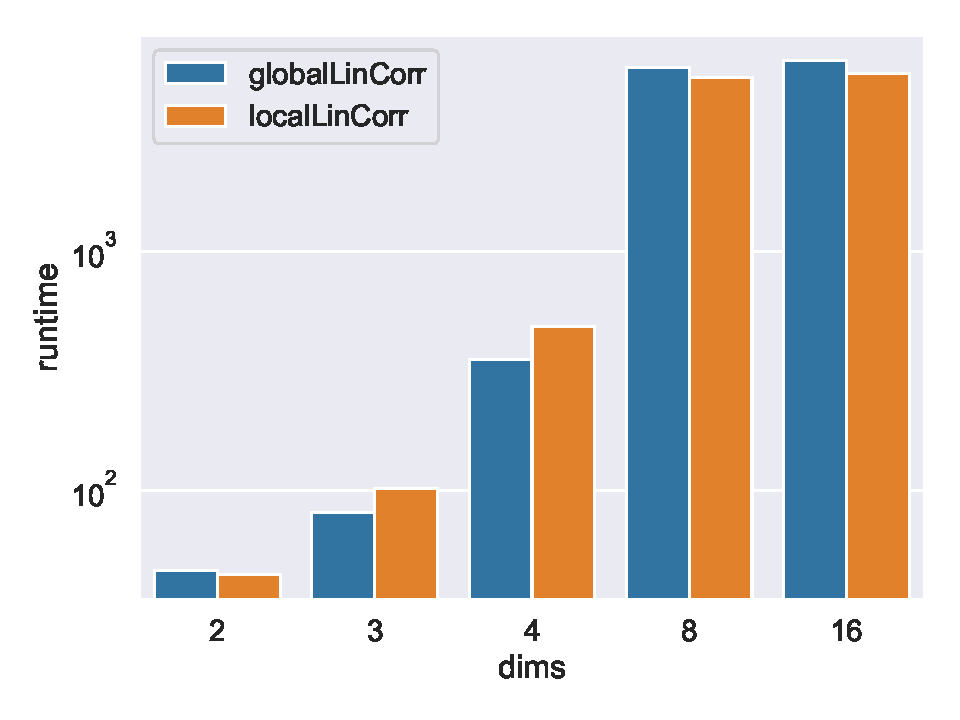
\includegraphics[width=0.8\textwidth]{evaluation/per_dims/Avg_Runtime_O10000_N5_pdims_log.pdf}
    \caption{Runtime in seconds w.r.t. the dimensionality of the whole data set - lower is better}
    \label{fig:eval_per_dims}
\end{figure}

\autoref{fig:eval_per_dims} shows a comparison of local and global algorithms average runtime performances with regards to expanding dimensionalities. This experiment was ran on data sets with 10000 objects and 5 percent noise with 2,3,4,8 and 16 dimensions. As expected the average runtime corresponding to the increasing dimensionality increases exponentially for both approaches, considering the runtime complexity of \gls{cash} and our algorithms complexity, which is also dominated by the complexity of \gls{cash}s $\mathcal{O}(2^d)$. Therefore it is sensible that both algorithms again perform comparably.
Since we capped the maximum runtime of each parameter search iteration to 2 hours we observe a stagnation of the runtime at 16 dimensions.\\

Summarized the experiments have demonstrated that the average runtime of our local approach is closely comparable to the default \gls{cash} with respect to number of points, amount of noise and dimensionalities. Therefore as assumed the overhead produced by the preprocessing component \gls{optics} and the postprocessing components \textit{Stitching} and \textit{Relabeling} are compensated by the faster runtime of the localized \gls{cash} ran on the partitioned subinterval of the data space. 
 
\subsection{Effectiveness}
To measure the clustering performance measures we picked the best parameter sets of the previous 500 iterations of parameter search of the efficiency evaluation for both local and global approach and stacked their \gls{ari} and \gls{nmi} scores up against each other. 

In our first setting we compared \gls{cash} and our algorithm according to the best \gls{ari} and \gls{nmi} scorings achieved during the parameter search with regards to the variable number of objects in data space. 
\begin{figure}[h]
    \centering
    \begin{minipage}[t]{.5\textwidth}
      \centering  
      \captionsetup{width=.9\linewidth}
      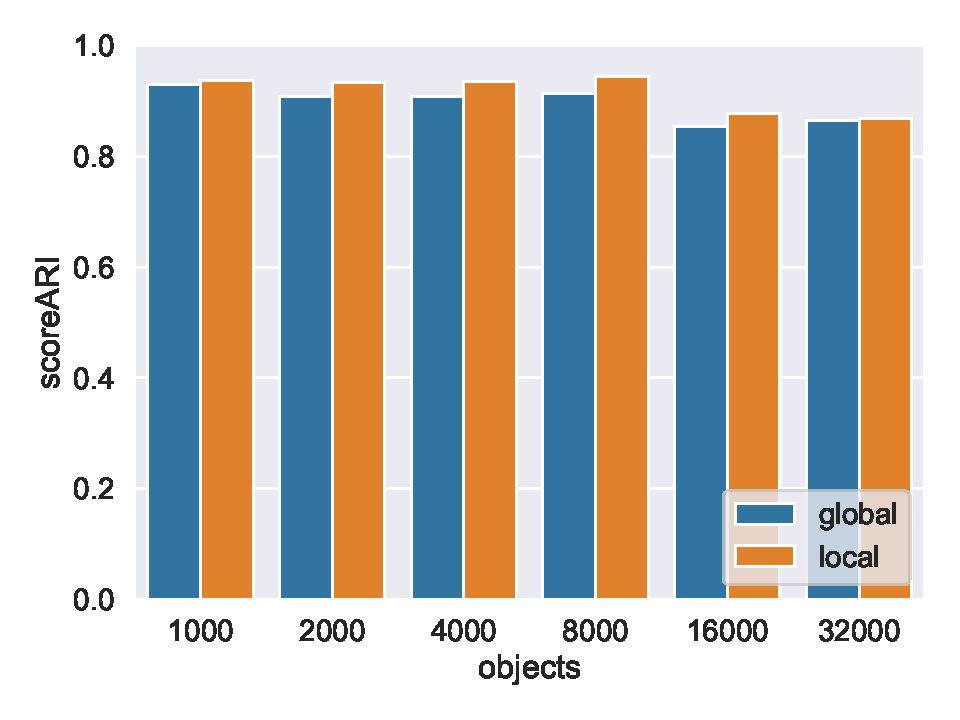
\includegraphics[width=\textwidth]{evaluation/per_objects/Best_ARI_3D_N5_pobjects_bar.pdf}
      \captionsetup{labelformat=empty}
      \caption{\gls{ari} score}
      \label{fig:ariperpts}
    \end{minipage}%
    \begin{minipage}[t]{.5\textwidth}
      \centering
      \captionsetup{width=.9\linewidth}
      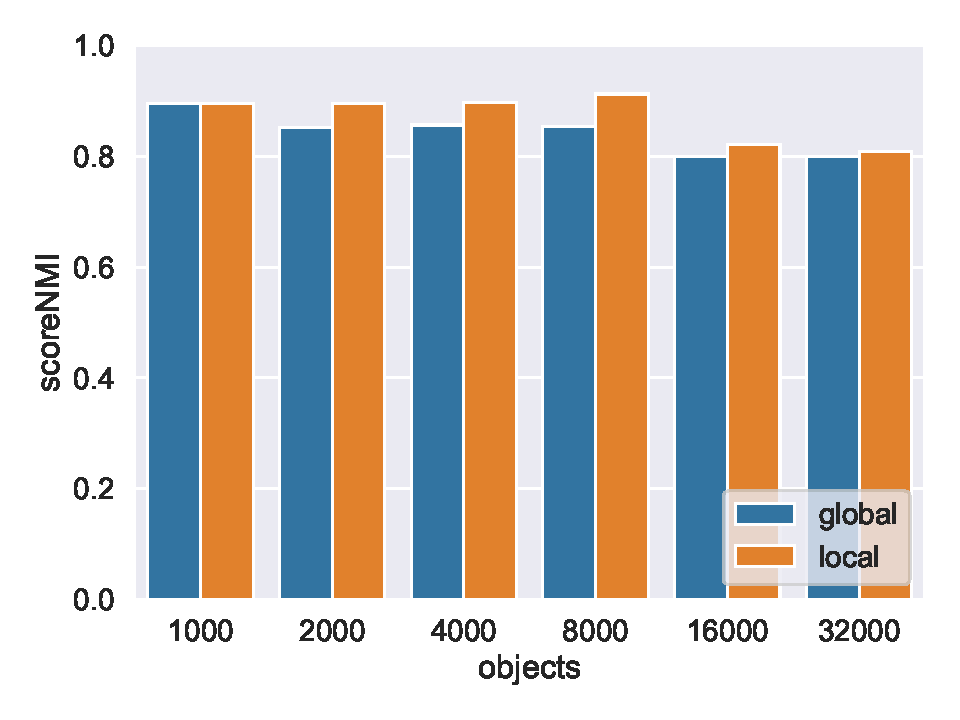
\includegraphics[width=\textwidth]{evaluation/per_objects/Best_NMI_3D_N5_pobjects_bar.pdf}
      \captionsetup{labelformat=empty}
      \caption{\gls{nmi} score}
      \label{fig:nmiperpts}
    \end{minipage}
    \caption{Scoring w.r.t the number of objects - higher is better}
    \label{fig:scoreperpts}
\end{figure}

\autoref{fig:scoreperpts} shows the comparison of the clustering scores achieved by both the local and global approach on the 3-dimensional data set with 5 percent noise with respect to six variable numbers of objects (1000, 2000, 4000, 8000, 16000, 32000). In terms of cluster size both algorithms perform comparably and score a similar \gls{ari} and \gls{nmi} score of over $0.8$. 

To assess the robustness of our clustering algorithm against noise, the second clustering performance evaluation was conducted on a data set with variable levels of noise. Given the best parameter settings achieved during the 500 iterations of parameter search in the efficiency evaluation step, we compared the \gls{ari} and the \gls{nmi} scores at different levels of noise of both algorithms against each other.
\begin{figure}[h]
    \centering
    \begin{minipage}[t]{.5\textwidth}
      \centering  
      \captionsetup{width=.9\linewidth}
      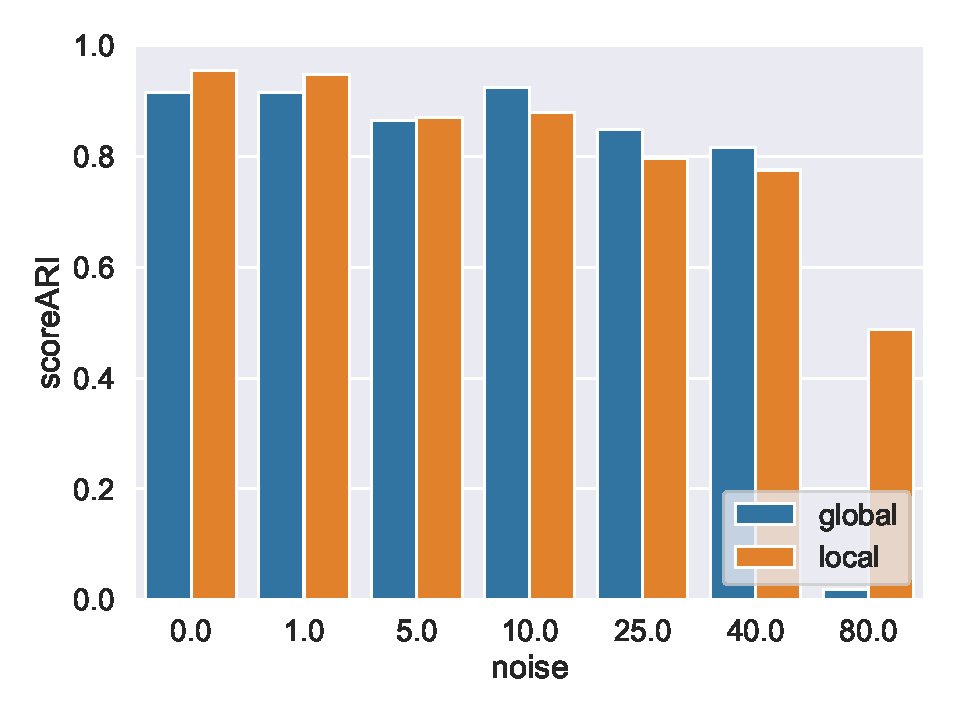
\includegraphics[width=\textwidth]{evaluation/per_noise/Best_ARI_3D_O10000_pnoise_bar.pdf}
      \captionof{figure}{\gls{ari} score w.r.t. amount of noise}
      \label{fig:ariperpts}
    \end{minipage}%
    \begin{minipage}[t]{.5\textwidth}
      \centering
      \captionsetup{width=.9\linewidth}
      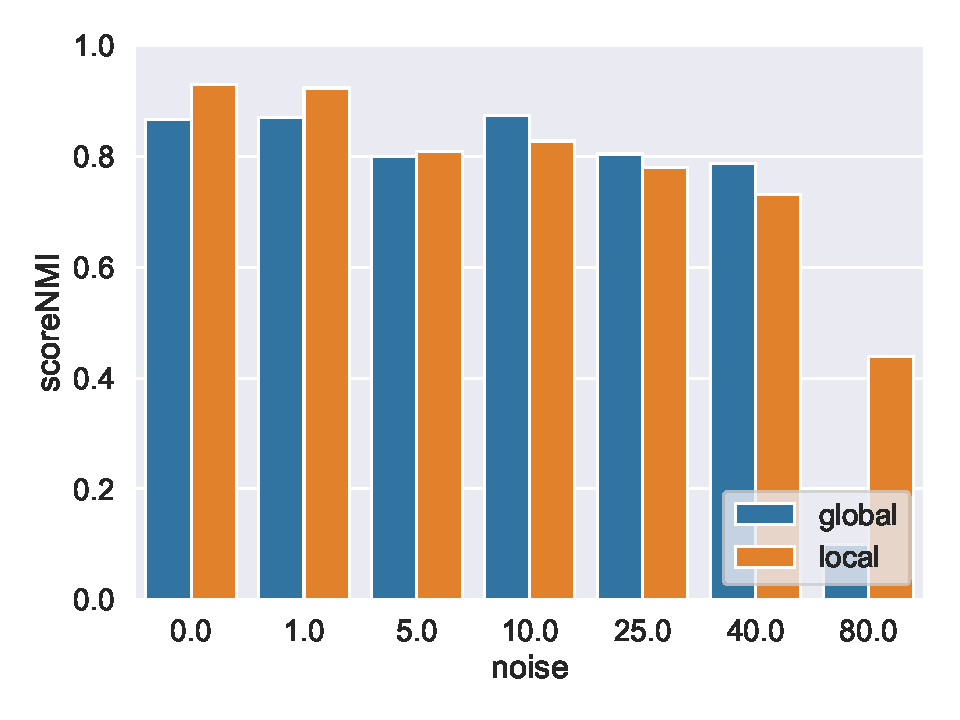
\includegraphics[width=\textwidth]{evaluation/per_noise/Best_NMI_3D_O10000_pnoise_bar.pdf}
      \captionof{figure}{\gls{nmi} score w.r.t. amount of noise}
      \label{fig:nmiperpts}
    \end{minipage}    
    \caption{Scoring w.r.t the noise percentage - higher is better}
    \label{fig:scorepernoise}
\end{figure}
The second experiment was ran on 3-dimensional base data sets with 10000 data points spread among all clusters with seven varying amounts of noise (0,1,5,10,25,40,80).
As \autoref{fig:scorepernoise} shows, the results of the clustering performance evaluation scoring between our algorithm and \gls{cash} remains close to eachother for low to mid levels of noise. At 80 percent noise our algorithm performs even better than the global \gls{cash}. This could be due to the high percentage of noise creating a high amount of candidate cells in parameter space, which are all considered as valid correlations in the global \gls{cash}. In contrast our approaches preprocessing via \gls{optics} might extract the underlying correlations, which are characterized by comparably more dense regions, first and and extract those local correlations via \gls{cash} faster and more accurately, since the partitions contain less noise and therefore the parameter space less candidates. These few prominent local correlations are then stitched together if similar enough and previously not considered points are relabeled, all together resulting in an quicker and more accurate global clustering compared to default \gls{cash} itself.

Our last clustering performance evaluation was targeted at the impact of the dimensionality of the data set. Here, we again picked the best parameter sets previously obtained during the runtime assessment to compare our algorithm with \gls{cash}.
\begin{figure}[h]
    \centering
    \begin{minipage}[t]{.5\textwidth}
      \centering  
      \captionsetup{width=.9\linewidth}
      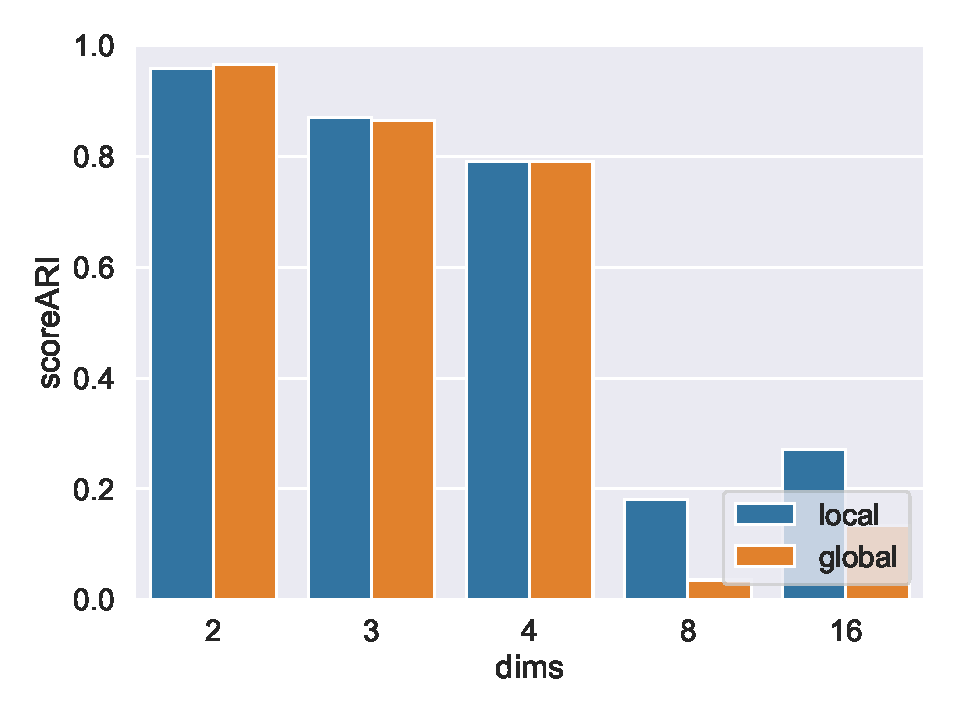
\includegraphics[width=\textwidth]{evaluation/per_dims/Best_ARI_O10000_N5_pdims_bar.pdf}
      \captionof{figure}{\gls{ari} score w.r.t. dimensionality}
      \label{fig:ariperpts}
    \end{minipage}%
    \begin{minipage}[t]{.5\textwidth}
      \centering
      \captionsetup{width=.9\linewidth}
      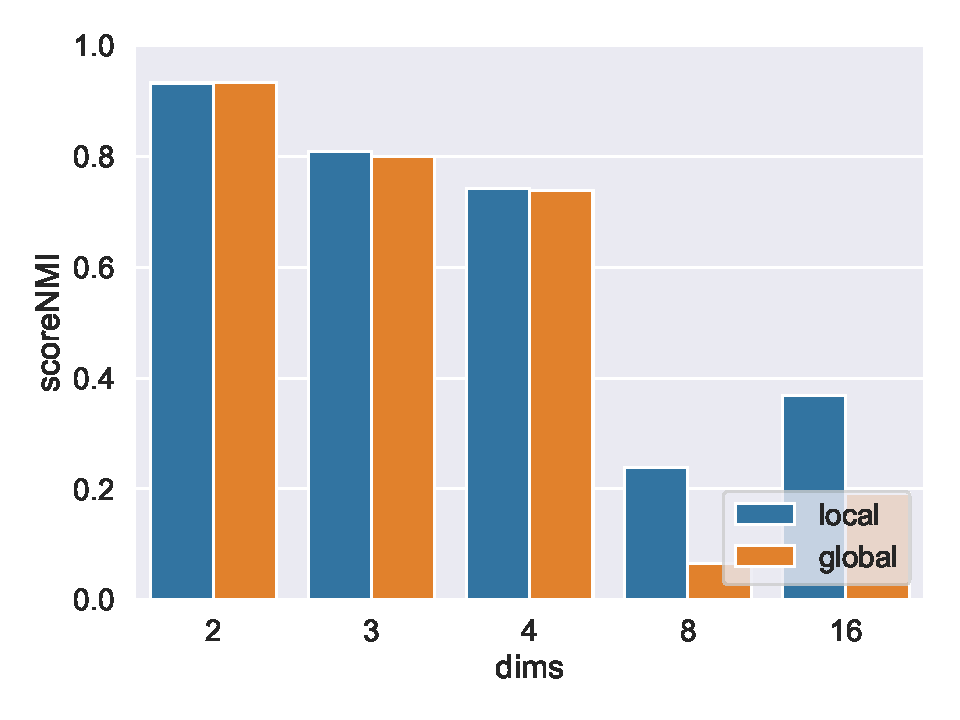
\includegraphics[width=\textwidth]{evaluation/per_dims/Best_NMI_O10000_N5_pdims_bar.pdf}
      \captionof{figure}{\gls{nmi} score w.r.t. dimensionality}
      \label{fig:nmiperpts}
    \end{minipage}
    \caption{Scoring w.r.t the dimensionality - higher is better}
    \label{fig:scoreperdims}
\end{figure}

\autoref{fig:scoreperdims} shows the different scores, \gls{ari} and \gls{nmi}, between both global and local approach applied on data sets with a fixed amount of 10000 data objects and 5 percent noise and a variable dimensionality of 2,3,4,8 and 16.
Note that since the evaluation of the runtime performance with regards to 8 and 16 dimensional data sets were stopped early due to time constraints, the optimal scorings of both 8 and 16 dimensional data sets are not representative for the optimal scores and will not be considered. 
The results of dimensions 2,3 and 4 show similar clustering results compared to both algorithms, however as the direction over these dimensions \gls{ari} and \gls{nmi} scores suggest, both \gls{cash} and our algorithm have an downwards trend in terms of clustering score with regards to dimensionality. This might be due to the fact, that the search space for \gls{cash} increases exponentially with respect to the dimensions, which increases the possible regions of interest (c.f. \autoref{fig:cash3d}). Instead of a single intersection in a point as a region of interest in 2-dimensional space, a 3-dimensional space for comparison has a complex curve as intersection which increases the amount of regions of interest considerably. This increased complexity might be the reason for the deteriorating performance in increasing dimensions. \todor{erwaehnt orginal cash das deswegen nicht?}\\

Summarized our experiments show, that our local approach yields similar results in various settings in terms of runtime as well as in terms of clustering performance compared to the original \gls{cash}, with an additional benefit of detecting locally dense correlations. \autoref{fig:clusterexample} shows an example of our algorithm with the local correlations clustering as an intermediate result and the relabeled global view of the correlation clustering. \autoref{fig:gclusterexample} shows the equivalent clustering performed by the default \gls{cash}. \todor{kann laenger sein}

\begin{figure}
    \centering
    \includegraphics{}
    \caption{Caption}
    \label{fig:clusterexample}
\end{figure}

\begin{figure}
    \centering
    \includegraphics{}
    \caption{Caption}
    \label{fig:gclusterexample}
\end{figure}

% \section{Parameters available and their impacts}
% As our algorithm depends on many components such as \gls{optics} and \gls{cash} which come with several parameters themselves. In this section we discuss their meaning and their impact for the clustering results.

% \subsection{Metrics: CosineSimiliarity(n1,n2), CosineSimiliarity(n1,n2) + EuclidianDistance(d) [2-3]}

% \subsection{Median vs.  Mean}

% \section{Results between Dense approach with stitching and Global approach}

% \section{Test on real world data set(s) [1]}

% %evtl. "Hyperparameter sensitivity" d.h. wie 'empfindlich' ist das verfahren bzgl. welchen Parameter Einstellungen?
\chapter{Conclusion}\label{ch:conclusion}
% Possible improvements by sampling (see \cite{opticsankerst1999optics})
In the present state of huge amounts of data acquisition in various fields,  such as medicine, economy and artificial intelligence, the task of detecting and extracting relevant subspace clusters continues to be highly relevant. However, the current implementations of correlation clustering algorithms only focus on the detection of either local correlation clusters or global correlation cluster and lack the means to find an agglomerated view of both during a single evaluation run. In this thesis, we reviewed existing Correlation Clustering approaches and highlighted their shortcomings concerning their target scope being only applicable for either local or global Correlation Clustering. 

As a solution, we proposed a novel approach for finding both scopes of clustering simultaneously by applying a density-based preprocessing step first and performing a Correlation Clustering algorithm on the resulting locally dense clusters afterwards. This intermediate result contains the local correlation clusters, which represents the local view of the Correlation Clustering. To create the global view, we combined the intermediate clusters by stitching them together if they are similar enough and relabelled all previously disregarded (not dense) points for completeness.

% Our empirical performance analysis in terms of clustering accuracy and runtime was conducted on three different experiments with regards to variable numbers of data objects, amounts of noise and dimensionalities, and additionally compared to the performance measures of its parent algorithm \gls{cash}.
To evaluate the performance in terms of clustering accuracy and runtime, we conducted three different settings for experiments with regards to the number of data objects, amount of noise and dimensionality, and compared those to the performance measures of its parent algorithm \gls{cash}. 
The runtime results yielded that on average, our algorithm, in each runtime setting, performs comparably to \gls{cash} and even gets a slight edge at a comparison in high noise levels. With regards to higher dimensionalities however, we were not able to retrieve representable performance measures due to time and processing power constraints. In terms of clustering performance, our tests, with the best parameter setting previously determined, revealed similar clustering scores as well, with our algorithm having an advantage at higher levels of noise again. However, the tests on the dimensionality also exposed, that both algorithms scale worse for increasing dimensions. At high dimensions, our algorithms best score paled in comparison to \gls{cash} due to the best parameter set being harder to determine since our algorithm requiring more parameters.

All things considered, our first empirical performance analysis yields that, in addition to providing both local and global Correlation Clustering, our algorithm performs equally well compared to original \gls{cash} in terms of the global view, and suggests promising performance in regards to correlation clusterings with arbitrary scopes.

\chapter{Future Work}\label{ch:futurework}
As the topic of correlation clustering with arbitrary scopes is by no means covered and is just at the beginning of the research, we want to provide suggestions for an outlook of potential future directions. 
% To provide an outlook of potential future directions gathered by ideation during the process of the creation of this work, we hope to motivate for future research and present the following contributions.

This work only covered a basic principle of assembling locally dense clusters with global correlation clustering via \gls{dbscan}/\gls{optics} and \gls{cash}. However, these components only served as quick and convenient building blocks to realize an implementation of said principle and by no means have to be the optimal solutions. For future work, we suggest to research and experiment with different, more advanced or modified components, e.g. using modified distance functions in \gls{dbscan}/\gls{optics} to cope for the Curse of Dimensionality, choosing a different Correlation Clustering method for improved correlation results or modifying the assembling method of the local correlation clusters.

As the in-depth evaluation of the impact to the performance measures for every single parameter is very extensive and was not possible in the frame of this thesis, a survey about the different parameters and their impacts with regards to local and global clustering results could be subject to future research.

Another path of future work targets the implementation of our algorithm itself as our work does not satisfy the need for high performance with regards to runtime we recommend to further research and elaborate on strategies to accelerate the execution time of our approach.



\appendix
\chapter{Results}

Results with Figures?

% Abbildungsverzeichnis (kann auch nach dem Inhaltsverzeichnis kommen)
\listoffigures

% Tabellenverzeichnis (kann auch nach dem Inhaltsverzeichnis kommen)
\listoftables

% Literaturverzeichnis
\bibliographystyle{dbstmpl}    % verwendet dbstmpl.bst
% alternative, vorinstallierte Stile sind z.B. plain oder abbrv
\bibliography{dbstmpl}         % verwendet dbstmpl.bib

\end{document}
